\documentclass[./dissertation.tex]{subfiles}

\begin{document}

    \contentchapter{Variational Autoencoders}

    \section{VAEs as Representation Learning}
    Like DML methods, variational autoencoders (VAEs) can be considered as a type of representation learning as VAEs also produce meaningful low-dimensional representations of input data. Even more specifically, both DML methods and VAEs contain component neural networks which serve as a mapping from the input space to the latent dimensionality. 
    
    \section{VAEs as a Generative Model}
    VAEs can also be thought of as a type of generative model. There are several ways to define and think about generative models. One way to consider generative models is that a generative model is a function $g$ which maps an input $X \in \mathcal{R}^{n}$ back to the space $\mathcal{R}^{n}$ (i.e. $g: \mathcal{R}^{n} \to \mathcal{R}^{n}$) such that the functions output is a reconstruction of the input ($g(X) = \hat{X}$). This explanation may not be applicable to all generative models (for instance, GANs do not reconstruct specific inputs though can be said to reconstruct training data), but is applicable to VAEs and helps provide an intuition for the broad goals of generative models.  \\
    
    Another way to describe generative models is a class of models which attempt to approximate the distribution of input data $P(X)$. For instance, one may attempt to approximate the distribution of all pictures of dogs $P(X_{dog})$ with a generative model. If the generative model is successful, one can approximately sample from $P(X_{dog})$ through the generative model. However, the challenge in this approach is that many classes of inputs, including images, are very high-dimensional, and thus it is difficult to learn it's distribution. For instance, a picture of a dog may be 256 pixels in both length and width and have 3 channels per pixel, in which case $X_{dog} \in \mathcal{R}^{256 \times 256 \times 3}$. It is clearly very difficult to learn a probability distribution of dimensionality ${256 \times 256 \times 3}$, so generative models must use a work around to contend with this dimensionality problem. VAEs, as we will discuss in the next section, use the architecture of the variational autoencoder to map the inputs to lower dimensional representations that are easier to model as distributions. 
    
    \section{VAEs as Autoencoders}
    We have stated that variational autoencoders look to learn the distribution of low-dimensional representations. To define the relationship between the high-dimensional inputs and low-dimensional representations, the authors use the autoencoder architecture. An autoencoder looks to enocde an input into a low-dimensional representation and decode the representation to a reconstruction of the input. Both the encoder and the decoder are paramaterized by neural networks. The autoencoder is generally trained using an expected reconstruction loss term \cite{bank2020autoencoders}. However, the VAE trains against a lower-bound of log-likelihood (that happens to include the a reconstruction loss term), which we discuss in the following section. Another key difference between autoencoders and VAEs is that autoencoders map an input $x \in \mathcal{R}^{D}$ to a vector $z \in \mathcal{R}^{d}$ while the VAE maps an input to a normal distribution (called the posterior) that is paramaterized by $\mu, \sigma \in \mathcal{R}^{d}$ from which a latent point is sampled. 
    
    \begin{figure}[h]
        \centering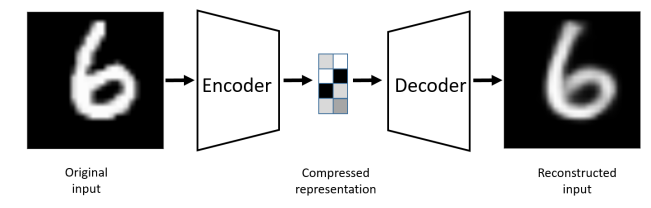
\includegraphics[width=0.5\textwidth]{figures/autoencoder.PNG}
        \caption{Diagram of autoencoders (Source: Bank et. al. 2020)}
        \label{Autoencoder Diagram}
    \end{figure}
    
    \section{The VAE Objective Function}
    To understand the derivation of the VAE objective function, it is first helpful to define the components of the VAE in their relationship to probability theory. The encoder of the VAE attempts to estimate the posterior distribution $p(z|x)$ so we will refer to it as $q_{\theta}(z|x)$, with $\theta$ referring to the parameters of the encoder network. Likewise, we refer to the decoder network as $p_{\phi}(x|z)$. $p(z)$ refers to a prior distribution that represents the prior beliefs about the latent variable's distribution (the choice of prior will be discussed in much greater detail in the following section). 
    
    The starting point deriving the evidence lower bound is computing the KL divergence between the approximated posterior distribution $q_{\theta}(z|x)$ and the real distribution $p(z|x)$. To compute the KL divergence between any two distributions, we use the following formula. 
    \begin{equation*}
        D_{KL}(q(x)|p(x)) = \int q(x)\log(\frac{q(x)}{p(x)}) = - \int q(x)\log(\frac{p(x)}{q(x)})
    \end{equation*}
    
    Thus, the distribution between $q_{\theta}(z|x)$ and $p(z|x)$ is
    \begin{equation*}
        D_{KL}(q_{\theta}(z|x)|p(z|x)) = - \int q_{\theta}(z|x)\log(\frac{p(z|x)}{q_{\theta}(z|x)})dz
    \end{equation*}
    
    Using Bayes Rule, we replace the unknown real posterior $p(z|x)$ with $\frac{p_{\phi}(x|z)p(z)}{p(x)}$
    \begin{equation*}
    \begin{aligned}
        D_{KL}(q_{\theta}(z|x)|p(z|x)) &= - \int q_{\theta}(z|x)\log(\frac{p_{\phi}(x|z)p(z)}{q_{\theta}(z|x)p(x)})dz \\
        &= - \int q_{\theta}(z|x)[\log(\frac{p_{\phi}(x|z)p(z)}{q_{\theta}(z|x)}) - \log(p(x))]dz \\
        &= - \int q_{\theta}(z|x)[\log(\frac{p_{\phi}(x|z)p(z)}{q_{\theta}(z|x)})dz + \int q_{\theta}(z|x)\log(p(x))dz \\
        &= - \int q_{\theta}(z|x)[\log(\frac{p_{\phi}(x|z)p(z)}{q_{\theta}(z|x)})dz + \log(p(x))dz \\
    \end{aligned}
    \end{equation*}
    
    Because KL divergence is always non-negative, we know the above expression is greater than or equal to zero. From this inequality, we can derive a lower bound of likelihood.
    \begin{equation*}
    - \int q_{\theta}(z|x)[\log(\frac{p_{\phi}(x|z)p(z)}{q_{\theta}(z|x)})dz + \log(p(x))dz \geq 0 \\
    \end{equation*}
    \begin{equation*}
    \begin{aligned}
    \log(p(x))dz &\geq \int q_{\theta}(z|x)[\log(\frac{p_{\phi}(x|z)p(z)}{q_{\theta}(z|x)})dz \\
    \log(p(x))dz &\geq \int q_{\theta}(z|x)[\log(\frac{p(z)}{q_{\theta}(z|x)})dz + \int q_{\theta}(z|x)p_{\phi}(x|z)dz \\
    \log(p(x))dz &\geq -D_{KL}(q_{\theta}(z|x)||p(z)) + E_{q_{\theta}(z|x)}(\log(p_{\phi}(x|z)))
    \end{aligned}
    \end{equation*}
    
    The right-hand side of the final line in the above derivation is the evidence lower bound (ELBO) which is used for the VAE loss function. In addition to representing the lower-bound of the log-likelihood, the ELBO can be considered as two loss terms that influence the VAE model in and of themselves. The KL-divergence term $-D_{KL}(q_{\theta}(z|x)||p(z))$ corresponds to the how close (as measured by the KL divergence metric) the approximated posterior distribution is to a prior distribution. The reconstruction loss term $\log(p_{\phi}(x|z)$ an be shown to be equivalent to the L2 norm. We drop the expected value as $z$ is sampled from the approximate posterior, allowing us to compute a monte carlo approximation over the distribution. Also recall that the decoder distribution $p_{\phi}(x|z) $ has a mean $\mu$ equivalent to the reconstructed input and a variance $\sigma$ of the identity matrix. The constants $c_{1}$ and $c_{2}$ can be ignored as they do not they do not impact the performance of the cost function. 
    
    \begin{equation*}
    \begin{aligned}
    \log(p_{\phi}(x|z)) &= \log(\frac{1}{\sqrt{2\pi}\sigma}e^{{-\frac{(x - \mu)^{2}}{2\sigma^{2}}}}) \\
    &= \log(\frac{1}{\sqrt{2\pi}}) - \log(\sigma) + \log(e^{{-\frac{(x - \mu)^{2}}{2\sigma^{2}}}}) \\
    &= c_{1} - \log(\sigma) - \frac{(x - \mu)^{2}}{2\sigma^{2}} \\
    &= c_{1} - \frac{(x - \mu)^{2}}{2} \\
    &= c_{1} - c_{2}(x - \mu)^{2} \\
    &\approx (x - \mu)^{2} \\
    \end{aligned}
    \end{equation*}
    
    \subsection{The VAE Prior Distribution and VampPrior}
    The prior distribution $p(z)$ in the KL divergence term is the unit gaussian $N(0, I)$ in most VAE implementations. Setting the prior as the unit gaussians has two distinct advantages. First, it is simple to compute a closed-form KL divergence between two gaussians \cite{}. Second, by choosing a prior distribution with a convex PDF, in sampling from the distribution during the generative process, we are less likely to sample points from that the decoder cannot provide quality reconstructions for \cite{}. \\
    
    The unit gaussian is not an ideal prior, however, in that it does not always capture the underlying structure of the data well. One proposed approach is the VAE with a VampPrior \cite{}, in which the prior is a dynamic mixture of gaussian components. More specifically, VampPrior defines a set number of pseudoinputs -- trainable paramaters of the same dimensionality of the inputs of which the encoded means and log-varaiances paramaterize the prior distribution. 

    \section{Combining Variational Autoencoders and Metric Learning}
    We present metric learning as a mechanism for cluster regularization in VAEs. To do this, we borrow from metric learning in creating a training sub-routine to augment the standard VAE training process. Specifically, the standard VAE loss of 
    \begin{equation*}
    \mathcal L(x)=\|x-\hat x\|^2+KL(q(z|x)\|p(z))    
    \end{equation*}
    is augmented to 
    \begin{equation*}
    \hat{\mathcal L}(x)=\mathcal{L}(x)+\mathcal{R}_p(x)    
    \end{equation*}
    where $\mathcal{R}_p(x)$ is a metric loss. We argue that adding a metric loss term within a the VAE provides theoretical advantages to a traditional metric learning system with respect to the clustering latent representations of a semi-supervised dataset for two reasons. This modified VAE can be viewed as both a modification of a VAE which can incorporate labelled data \emph{or} as a new metric form of metric loss which benefits from unsupervised data. We take the latter perspective to propose and experimentally evaluate claims regarding the Metric VAEs benefits.
    
    We hypothesize that adding a metric loss term within the VAE provides theoretical advantages to a traditional metric learning system with respect to the clustering latent representations of a semi-supervised dataset for two reasons. 

    First, metric learning systems and VAEs both contain encoder functions $f$, but only VAEs contain a decoder function $g$. Having a decoder function $g$ allows us to compute a reconstruction error between the input $X$ and the reconstruction $\hat x=f(g(x))$. We claim that this reconstruction error helps clustering of unlabelled data because as while the decoder learns which areas of the latent space correspond to output phenoytpes, the encoder learns where data should be mapped to in the latent space, meaning data that appears to be similar is mapped closer together in latent space. Additionally, the presence of the decoder function $g$ allows us to build reconstructions of points in the latent space, which is a functionality that may be helpful to experts using the system.
    
    Second, latent points in metric learning systems are not constrained by a prior, while latent points in VAEs are. Specifically, the latent points are sampled from the posterior distributions; the distance between the posterior distributions and the prior distribution is minimized through the KL divergence term of VAE loss function. We have shown that the prior can be not only the unit Gaussian, but a mixture of $n$ gaussians created dynamically as the posteriors of $n$ pseudo-inputs. We claim that by modifying the prior, we can induce biases in the prior based on what we know about the dataset to encourage more accurate clustering patterns. For instance, knowing that there are $n$ many classes in a dataset (i.e. $n=10$ for the MNIST handwritten digets dataset), a prior distribution consisting of $n$ gaussians may best capture the underlying structure of the data. This hypothesis is also tested experimentally in section 5.

    

\end{document}
